\subsection*{Приложение}


Образец 2 помещён внутрь катушки, входящей в состав генератора. Генератор представляет собой часть индикаторной установки 1, магнитное поле в образце создаётся с помощью электромагнита 4. Основное магнитное поле создаётся с помощью катушек 5, питаемых постоянным током. Величина тока регулируется реостатом $R$ и измеряется амперметром $A$. Небольшое дополнительное поле возбуждается модулирующими катушками 6, присоединёнными к сети переменного тока через трансформатор 3. Напряжение на катушках регулируется потенциометром 8.


Основной частью установки является генератор слабых колебаний. Он представлет собой усилитель с положительной обратной связью, благодаря которой поддерживается непрерывная генерация. Катушка с образцом и находящийся в ящике 1 конденсатор переменной ёмкости образуют сеточный контур генератора. Ёмкость конденсатора можно менять, поворачивая лимб 7. При наступлении ЯМР поглощение энергии в образце увеличивается, добротность сеточного контура падает и амплитуда генерации уменьшается. Высокочастотный сигнал с генератора усиливается и детектируется.


Детектирование сигнала ЯМР осуществляется с помощью промышленного прибора. Модуляция магнитного поля осуществляется с помощью небольшой катушки, частота модуляции $\approx$ 50 Гц. В зазоре электромагнита устанавливается холловский измеритель магнитного поля, а измерения ЯМР проводятся на резине (измеряется ЯМР на протонах), тефлоне (в состав входит фтор) и тяжелой воде.


Сигнал ядерного магнитного резонанса наблюдается на экране осциллографа. На рисунке 3  изображен временной ход магнитного поля электромагнита. Как уже отмечалось, постоянная часть поля создается основными, а переменная -- модулируюшими катушками. При правильной настройке установки магнитное поле колеблется около резонансного значения, пересекая его два раза за каждый период изменения тока в модулирующих катушках. Как видно из рисунке 3, время, проходящее между следуюшими друг за другом пересечениями, одинаково при точном равенстве постоянного магнитного поля резонансному значению $B_{0}$ (рис. 3а) и различается при неточном их соответствии (рис. 3б) основной составляющей магнитного поля.


\begin{figure}[h]
    \centering
    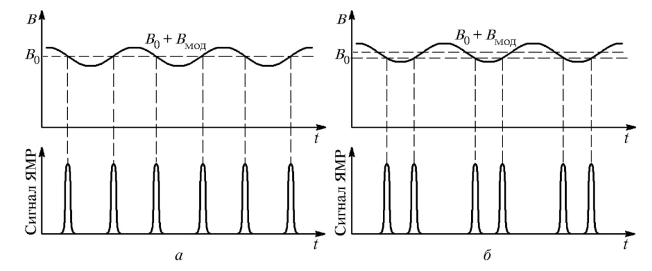
\includegraphics[width=0.5\textwidth]{ft.png}
    \caption{Временная зависимость магнитного поля и сигнала ядерного магнитного резонанса.}
    %\label{fig:}
\end{figure}
